\documentclass{beamer}

\usepackage{beamerthemesplit}
\usepackage{graphicx}
\usepackage{color, natbib, hyperref}
\usepackage{bibentry}
\usepackage[export]{adjustbox}% http://ctan.org/pkg/adjustbox
\usepackage{multicol}

\nobibliography*

% define colors
\definecolor{jblue}  {RGB}{20,50,100}
\definecolor{ngreen} {RGB}{98,158,31}

%theme

\usetheme{boxes} 
%\usecolortheme{seahorse} 
\setbeamertemplate{items}[default] 
%\setbeamercovered{transparent}
\setbeamertemplate{blocks}[rounded]
\setbeamertemplate{navigation symbols}{} 
% set the basic colors
\setbeamercolor{palette primary}   {fg=black,bg=white}
\setbeamercolor{palette secondary} {fg=black,bg=white}
\setbeamercolor{palette tertiary}  {bg=jblue,fg=white}
\setbeamercolor{palette quaternary}{fg=black,bg=white}
\setbeamercolor{structure}{fg=jblue}
\setbeamercolor{titlelike}{bg=jblue,fg=white}
\setbeamercolor{frametitle}{bg=jblue!10,fg=jblue}
\setbeamercolor{cboxb}{fg=black,bg=jblue}
\setbeamercolor{cboxr}{fg=black,bg=red}

% reduce space before/after equations
\expandafter\def\expandafter\normalsize\expandafter{%
    \normalsize
    \setlength\abovedisplayskip{1pt}
    \setlength\belowdisplayskip{1pt}
    \setlength\abovedisplayshortskip{1pt}
    \setlength\belowdisplayshortskip{1pt}
}

% set colors for itemize/enumerate
\setbeamercolor{item}{fg=ngreen}
\setbeamercolor{item projected}{fg=white,bg=ngreen}

% set colors for blocks
\setbeamercolor{block title}{fg=ngreen,bg=white}
\setbeamercolor{block body}{fg=black,bg=jblue!10}

% set colors for alerted blocks (blocks with frame)
\setbeamercolor{block alerted title}{fg=white,bg=jblue}
\setbeamercolor{block alerted body}{fg=black,bg=jblue!10}
\setbeamercolor{block alerted title}{fg=white,bg=dblue!70} % Colors of the highlighted block titles
\setbeamercolor{block alerted body}{fg=black,bg=dblue!10} % Colors of the body of highlighted blocks

% set the fonts
\usefonttheme{professionalfonts}

\setbeamerfont{section in head/foot}{series=\bfseries}
\setbeamerfont{block title}{series=\bfseries}
\setbeamerfont{block alerted title}{series=\bfseries}
\setbeamerfont{frametitle}{series=\bfseries}
\setbeamerfont{frametitle}{size=\Large}
\setbeamerfont{block body}{series=\mdseries}
\setbeamerfont{caption}{series=\mdseries}
\setbeamerfont{headline}{series=\mdseries}


% set some beamer theme options
\setbeamertemplate{title page}[default][colsep=-4bp,rounded=true]
\setbeamertemplate{sections/subsections in toc}[square]
\setbeamertemplate{items}[circle]
\setbeamertemplate{blocks}[width=0.0]
\beamertemplatenavigationsymbolsempty

% Custom colors
\usepackage{color}
%\definecolor{deepblue}{rgb}{0,0,0.5}
%\definecolor{deepred}{rgb}{0.6,0,0}
%\definecolor{deepgreen}{rgb}{0,0.5,0}
\definecolor{Code}{rgb}{0,0,0}
\definecolor{Decorators}{rgb}{0.5,0.5,0.5}
\definecolor{Numbers}{rgb}{0.5,0,0}
\definecolor{MatchingBrackets}{rgb}{0.25,0.5,0.5}
\definecolor{Keywords}{rgb}{0,0,1}
\definecolor{self}{rgb}{0,0,0}
\definecolor{Strings}{rgb}{0,0.63,0}
\definecolor{Comments}{rgb}{0,0.63,1}
\definecolor{Backquotes}{rgb}{0,0,0}
\definecolor{Classname}{rgb}{0,0,0}
\definecolor{FunctionName}{rgb}{0,0,0}
\definecolor{Operators}{rgb}{0,0,0}

% Default fixed font does not support bold face
\usepackage[utf8]{inputenc}
\DeclareFixedFont{\ttb}{T1}{txtt}{bx}{n}{12} % for bold
\DeclareFixedFont{\ttm}{T1}{txtt}{m}{n}{12}  % for normal

% Python style for highlighting
\usepackage{listings}
\newcommand\pythonstyle{\lstset{
language=Python,
%numbers=left,
%numberstyle=\footnotesize,
%numbersep=1em,
xleftmargin=1em,
framextopmargin=2em,
framexbottommargin=2em,
showspaces=false,
showtabs=false,
showstringspaces=false,
frame=l,
tabsize=4,
% Basic
basicstyle=\ttfamily\tiny,
otherkeywords={self},             % Add keywords here
keywordstyle={\color{Keywords}\bfseries},
% Comments
commentstyle=\color{Comments}\slshape,
%% Strings
stringstyle=\color{Strings},
morecomment=[s][\color{Strings}]{"""}{"""},
morecomment=[s][\color{Strings}]{'''}{'''},
% keywords
morekeywords={import,from,class,def,for,while,if,is,in,elif,else,not,and,or,print,break,continue,return,True,False,None,access,as,,del,except,exec,finally,global,import,lambda,pass,print,raise,try,assert},
keywordstyle={\color{Keywords}\bfseries},
% additional keywords
morekeywords={[2]@invariant,pylab,numpy,np,scipy},
keywordstyle={[2]\color{Decorators}\slshape},
emph={self},
emphstyle={\color{self}\slshape},
frame=tb,                         % Any extra options here
showstringspaces=false            % 
}}

% Python environment
\lstnewenvironment{python}[1][]
{
\pythonstyle
\lstset{#1}
}
{}

% Python for external files
\newcommand\pythonexternal[2][]{{
\pythonstyle
\lstinputlisting[#1]{#2}}}

% Python for inline
\newcommand\pythoninline[1]{{\pythonstyle\lstinline!#1!}}



% Math macros
\newcommand{\cD}{{\mathcal D}}
\newcommand{\cF}{{\mathcal F}}
\newcommand{\todo}[1]{{\color{red}{TO DO: \sc #1}}}

\newcommand{\reals}{\mathbb{R}}
\newcommand{\integers}{\mathbb{Z}}
\newcommand{\naturals}{\mathbb{N}}
\newcommand{\rationals}{\mathbb{Q}}

\newcommand{\ind}[1]{1_{#1}} % Indicator function
\newcommand{\pr}{\mathbb{P}} % Generic probability
\newcommand{\ex}{\mathbb{E}} % Generic expectation
\newcommand{\var}{\textrm{Var}}
\newcommand{\cov}{\textrm{Cov}}

\newcommand{\normal}{N} % for normal distribution (can probably skip this)
\newcommand{\eps}{\varepsilon}
\newcommand\independent{\protect\mathpalette{\protect\independenT}{\perp}}
\def\independenT#1#2{\mathrel{\rlap{$#1#2$}\mkern2mu{#1#2}}}

\newcommand{\convd}{\stackrel{d}{\longrightarrow}} % convergence in distribution/law/measure
\newcommand{\convp}{\stackrel{P}{\longrightarrow}} % convergence in probability
\newcommand{\convas}{\stackrel{\textrm{a.s.}}{\longrightarrow}} % convergence almost surely

\newcommand{\eqd}{\stackrel{d}{=}} % equal in distribution/law/measure
\newcommand{\argmax}{\arg\!\max}
\newcommand{\argmin}{\arg\!\min}


\mode<presentation>

\title[permute]{permute: A Python Package for Randomization Inference}
\author{Kellie Ottoboni}
\institute[]{Department of Statistics, UC Berkeley\\Berkeley Institute for Data Science}
\date{June 14, 2016}

\begin{document}

\frame{
\titlepage
\vfill
\begin{columns}[T]
\begin{column}{.5\textwidth}
\begin{center}
\vspace{25pt}

\includegraphics[width=\textwidth]{logo/dept1.pdf}
\end{center}
\end{column}
\begin{column}{.3\textwidth}
\end{column}
\begin{column}{.3\textwidth}
\begin{center}

\includegraphics[width=0.9\textwidth]{logo/BIDS.png}
\end{center}
\end{column}
\end{columns}
}

\AtBeginSection[]
{
   \begin{frame}
       \frametitle{Outline}
       \tableofcontents[currentsection]
   \end{frame}
}



\section[Introduction]{Introduction}


\frame{
History of randomization inference
- fisher
- neyman model
}


\frame{
R has several packages for randomization inference.
\begin{multicols}{2}
\begin{itemize}
\item \texttt{ri} %by Peter Aronow and Cyrus Samii

%{\tiny\textit{``This package provides a set of tools for conducting exact or approximate inference for randomized experiments of arbitrary design. The primary functionality of the package is in the generation, manipulation and use of permutation matrices implied by given experimental designs...''}\par}
\item \texttt{RItools} %by Mark Fredrickson

%{\tiny\textit{``The RItools package implements useful functions for implementing randomization inference based statistical tests. The package provides tools for testing balance of observed covariates in observational studies using the methodology of:...The package also provides outcome analysis of simple or block randomized trials (or matched observational studies) based on user defined models and test statistics.''}\par}
\item \texttt{coin} %by Torsten Hothorn, Kurt Hornik, Mark A. van de Wiel, and Achim Zeileis

%{\tiny\textit{The R package coin implements a unified approach to permutation tests providing a huge class of independence tests for nominal, ordered, numeric, and censored data as well as multivariate data at mixed scales. Based on a rich and flexible conceptual framework that embeds different permutation test procedures into a common theory, a computational framework is established in coin that likewise embeds the corresponding R functionality in a common S4 class structure with associated generic functions.}\par}
\item \texttt{perm} %by Michael Fay

%{\tiny\textit{The package has three main functions, to perform linear permutation tests. These tests are tests where the test statistic is the sum of the product of a covariate (usually group indicator) and the scores.}\par}
\end{itemize}
\end{multicols}
\vspace{20pt}
In Python, statistics packages are limited.
\begin{multicols}{2}
\begin{itemize}
\item \texttt{numpy.random} %generates random variables from common distributions
\item \texttt{scipy.stats} % computes moments, evaluates distribution functions, and generates random variables from common distributions and does common tests
\item \texttt{StatsModels} %is a Python module that provides classes and functions for the estimation of many different statistical models, as well as for conducting statistical tests, and statistical data exploration. 
\item \texttt{scikit-learn} %is a module for machine learning 
\end{itemize}
\end{multicols}

}


\frame{
\frametitle{Python is gaining popularity for doing data analysis}
PYPL Popularity of Programming Language Index, Worldwide

\begin{center}
\begin{figure}[htbp]
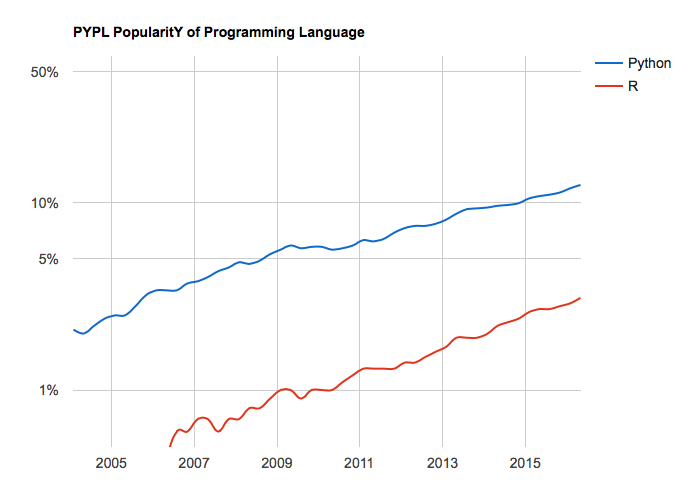
\includegraphics[width=\textwidth]{google_trends/pypl.png}
\end{figure}
{Keyword: how to}
\end{center}

}

\frame{
\frametitle{Python is gaining popularity for doing data analysis}
Google trends on May 22, 2016

\begin{center}
\begin{figure}[htbp]
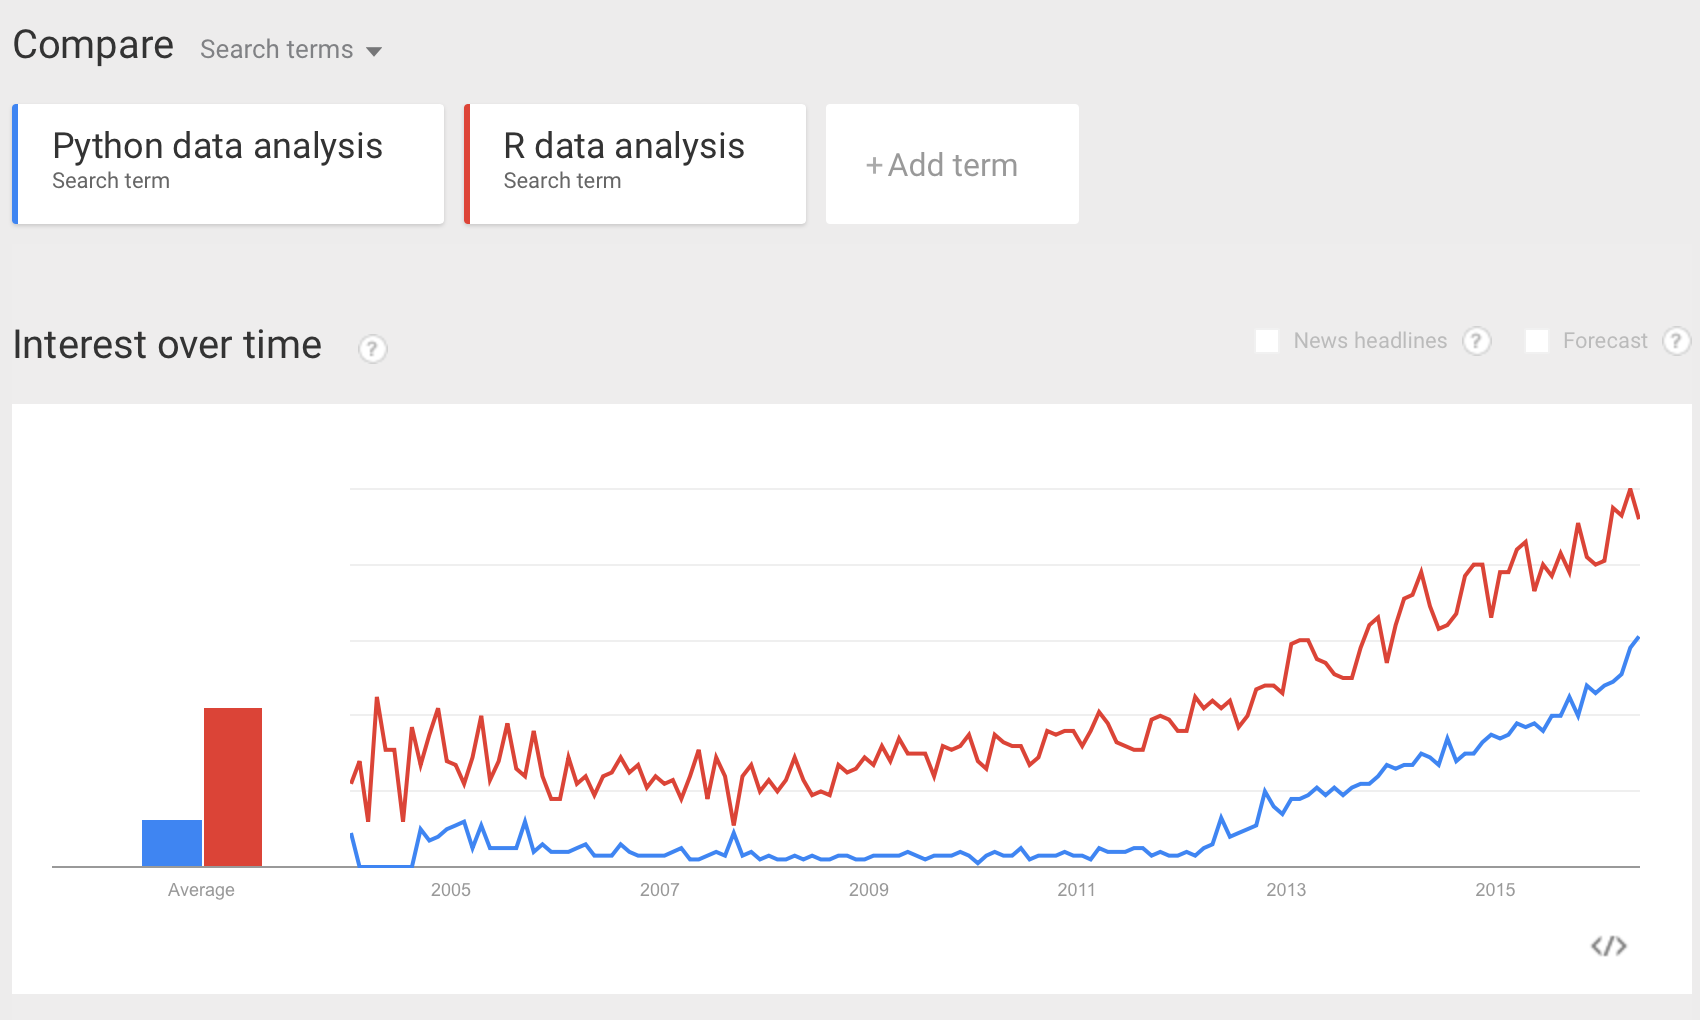
\includegraphics[width=\textwidth]{google_trends/dataanalysis}
\end{figure}
{Keyword: data analysis}
\end{center}

}

\frame{
\frametitle{Python is gaining popularity for doing data analysis}

Google trends on May 22, 2016
\begin{center}
\begin{figure}[htbp]
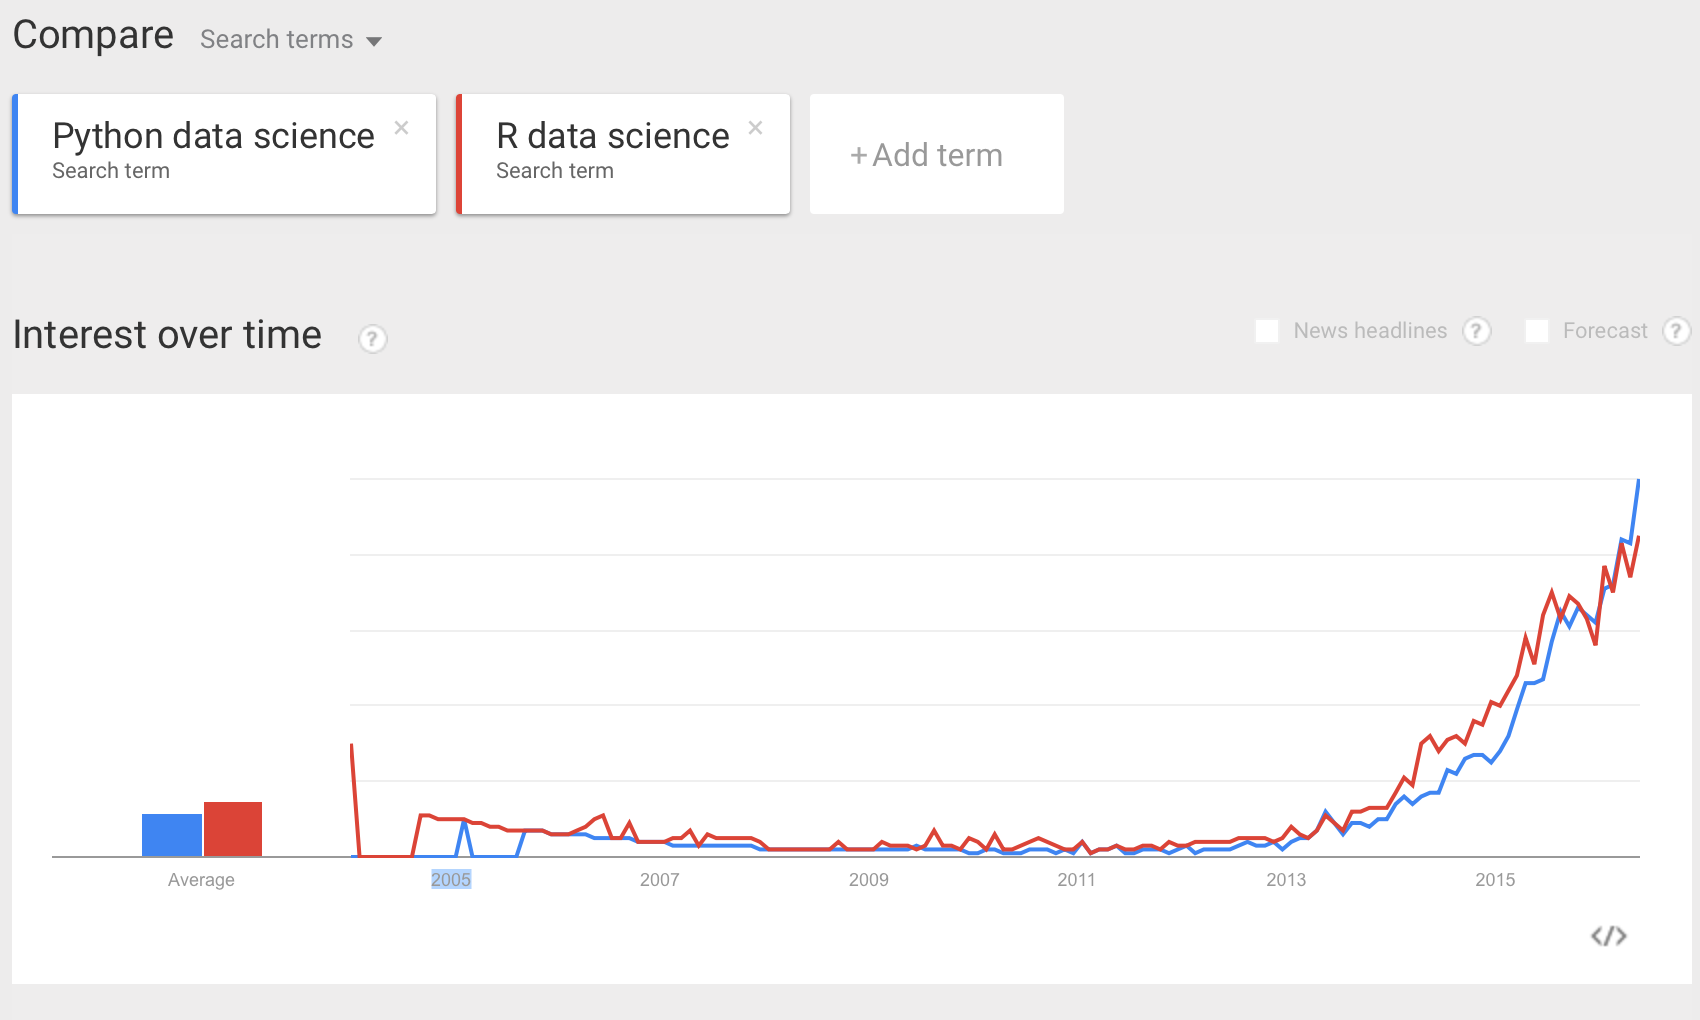
\includegraphics[width=\textwidth]{google_trends/datascience}
\end{figure}
{Keyword: data science}
\end{center}

}



\section[Examples]{Examples}
\subsection[Teaching evaluations]{Gender bias in teaching evaluations}


\frame
{
  \frametitle{ ~}
 \begin{center}
 \Large{ Student evaluations of teachers (SET) are used to} \\
  \begin{itemize}
  \item Quantify teaching effectiveness
  \item Compare instructors across courses
  \item Make hiring, firing, and promotion decisions  
  \end{itemize}
  \vfill
Are SET a valid measure of teaching effectiveness?
\end{center}
}


\frame
{
  \frametitle{ ~}
  \begin{center}
  \Huge{No!}
  \end{center}
\Large

We reanalyzed data from \cite{macnell2014whats}.
\begin{center}
\begin{itemize}
\itemsep 15pt
\item Students randomized to 4 online sections of a course
\item In two sections, the TAs swapped identities
\item Female-identified TA was rated lower on average in all categories
\end{itemize}
\end{center}
}


\frame{
\frametitle{Neyman-Rubin model, generalized}
Student $i$ is represented by a ticket with $4$ numbers, their response to each ``treatment.''

\begin{align*}
r_{ijk} &= \text{ SET given by student }i\text{ to instructor }j \\
&\text{ when they appear to have gender }k
\end{align*}
$$i = 1, \dots, N; \qquad j = 1,2; \qquad k \in \{ \text{male, female} \}$$

\vspace{10pt}
Numbers are fixed; randomization reveals one of the numbers. \\
\vspace{10pt}
Assume non-interference: each student's response depends only on that student's treatment. \\
\vspace{10pt}
If gender doesn't matter,
$$r_{ij\text{male}} = r_{ij\text{female}}.$$
}


\begin{frame}[fragile]
\begin{python}
# initialize PRNG
rs = np.random.RandomState(seed=1)
reps=10**5

ratings = macnell2014()

# Ratings vs reported instructor gender (difference in means)
(p, t, distr) = stratified_two_sample(ratings['overall'][ratings.taidgender==1],                                      ratings['overall'][ratings.taidgender==0], 
                      ratings['tagender'][ratings.taidgender == 1], 
                      ratings['tagender'][ratings.taidgender == 0],
                      alternative = "two-sided", stat='mean', seed = rs, 
                      reps = reps, keep_dist = True)
print 'Overall rating:'
print 'Difference in means:', t
print 'P-value (two-sided):', np.round(p, 5), "\n"\end{python}
\end{frame}


\frame
{
  \frametitle{Results}

\begin{table}
\begin{tabular}{r|crr}
\textbf{Characteristic} & \textbf{M-F} & \textbf{perm} $P$ & \textbf{t-test} $P$ \\
\hline
Overall & 0.47 & 0.12 & 0.128\\
Caring & 0.52 & 0.10 & 0.071\\
%Clear & 0.41 & 0.29 & NA \\
%Communicate & 0.57 & 0.07 & NA \\
Consistent & 0.47 & 0.21 & 0.045 \\ % The test stat didn't match Philip's talk...go back to notebook and paper
Enthusiastic & 0.57 & 0.06 & 0.112 \\
Fair & 0.76 & 0.01 & 0.188 \\
Feedback & 0.47 & 0.16 & 0.054 \\
Helpful & 0.46 & 0.17 & 0.049 \\
Knowledgeable & 0.35 & 0.29 & 0.038 \\
Praise & 0.67 & 0.01 & 0.153 \\
Professional & 0.61 & 0.07 & 0.124 \\
Prompt & 0.80 & 0.01 & 0.191 \\
Respectful & 0.61 & 0.06 & 0.124 \\
Responsive & 0.22 & 0.48 & 0.013
\end{tabular}
\end{table}

}


\subsection[Salt and mortality]{Salt and mortality at the level of nations}

\frame{
salt and mortality
}


\subsection[Inter-rater reliability]{Inter-rater reliability}
\frame{
NSGK IRR stuff
\citet{millman2016case}
}

\section[Software and Statistics]{The role of software development in Statistics}

\frame{
Reproducibility crisis:
\begin{itemize}
\item Why Most Published Research Findings Are False (Ioannidis, 2005)
\item 30--50\%\todo{} of studies fail to replicate (\todo{cite})
\end{itemize}
}

\frame{
\textbf{Why?} 

\begin{itemize}
\item File drawer problem
\item Publication bias: positive findings are more likely to get published
\item P-hacking and trying many models before reporting one
\item Inappropriate statistical tests
\end{itemize}

Randomization inference may ameliorate the last problem
}

\frame{
\frametitle{Download \texttt{permute}!}
\begin{figure}[htbp]
\begin{center}
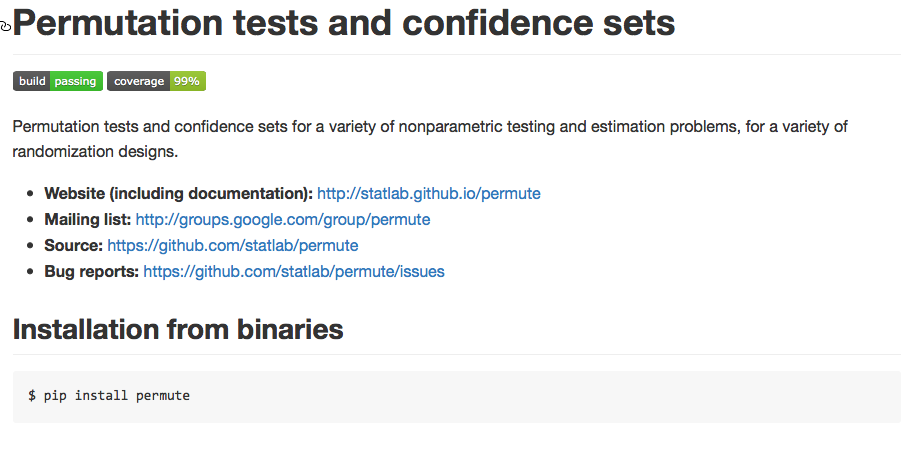
\includegraphics[width=\textwidth]{github/permute}
\end{center}
\end{figure}


\url{https://github.com/statlab/permute}
}


\frame{
\frametitle{Collaborators}
\begin{figure}[htbp]
\begin{center}
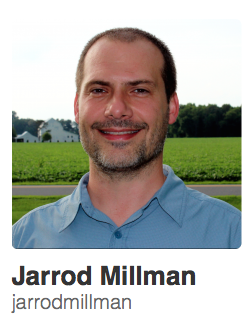
\includegraphics[width = 0.3\textwidth, valign=t]{github/jarrodmillman} 

\includegraphics[width = 0.3\textwidth, valign=t]{github/pbstark} 

\includegraphics[width = 0.3\textwidth, valign=t]{github/stefanv} 
\end{center}
\end{figure}

}

\begin{frame}
\frametitle{References}
\tiny
\bibliographystyle{plainnat}
\bibliography{refs}
\itemize
\end{frame}


\end{document}
